\documentclass[twoside]{book}

% Packages required by doxygen
\usepackage{fixltx2e}
\usepackage{calc}
\usepackage{doxygen}
\usepackage[export]{adjustbox} % also loads graphicx
\usepackage{graphicx}
\usepackage[utf8]{inputenc}
\usepackage{makeidx}
\usepackage{multicol}
\usepackage{multirow}
\PassOptionsToPackage{warn}{textcomp}
\usepackage{textcomp}
\usepackage[nointegrals]{wasysym}
\usepackage[table]{xcolor}

% Font selection
\usepackage[T1]{fontenc}
\usepackage[scaled=.90]{helvet}
\usepackage{courier}
\usepackage{amssymb}
\usepackage{sectsty}
\renewcommand{\familydefault}{\sfdefault}
\allsectionsfont{%
  \fontseries{bc}\selectfont%
  \color{darkgray}%
}
\renewcommand{\DoxyLabelFont}{%
  \fontseries{bc}\selectfont%
  \color{darkgray}%
}
\newcommand{\+}{\discretionary{\mbox{\scriptsize$\hookleftarrow$}}{}{}}

% Page & text layout
\usepackage{geometry}
\geometry{%
  a4paper,%
  top=2.5cm,%
  bottom=2.5cm,%
  left=2.5cm,%
  right=2.5cm%
}
\tolerance=750
\hfuzz=15pt
\hbadness=750
\setlength{\emergencystretch}{15pt}
\setlength{\parindent}{0cm}
\setlength{\parskip}{3ex plus 2ex minus 2ex}
\makeatletter
\renewcommand{\paragraph}{%
  \@startsection{paragraph}{4}{0ex}{-1.0ex}{1.0ex}{%
    \normalfont\normalsize\bfseries\SS@parafont%
  }%
}
\renewcommand{\subparagraph}{%
  \@startsection{subparagraph}{5}{0ex}{-1.0ex}{1.0ex}{%
    \normalfont\normalsize\bfseries\SS@subparafont%
  }%
}
\makeatother

% Headers & footers
\usepackage{fancyhdr}
\pagestyle{fancyplain}
\fancyhead[LE]{\fancyplain{}{\bfseries\thepage}}
\fancyhead[CE]{\fancyplain{}{}}
\fancyhead[RE]{\fancyplain{}{\bfseries\leftmark}}
\fancyhead[LO]{\fancyplain{}{\bfseries\rightmark}}
\fancyhead[CO]{\fancyplain{}{}}
\fancyhead[RO]{\fancyplain{}{\bfseries\thepage}}
\fancyfoot[LE]{\fancyplain{}{}}
\fancyfoot[CE]{\fancyplain{}{}}
\fancyfoot[RE]{\fancyplain{}{\bfseries\scriptsize Generated by Doxygen }}
\fancyfoot[LO]{\fancyplain{}{\bfseries\scriptsize Generated by Doxygen }}
\fancyfoot[CO]{\fancyplain{}{}}
\fancyfoot[RO]{\fancyplain{}{}}
\renewcommand{\footrulewidth}{0.4pt}
\renewcommand{\chaptermark}[1]{%
  \markboth{#1}{}%
}
\renewcommand{\sectionmark}[1]{%
  \markright{\thesection\ #1}%
}

% Indices & bibliography
\usepackage{natbib}
\usepackage[titles]{tocloft}
\setcounter{tocdepth}{3}
\setcounter{secnumdepth}{5}
\makeindex

% Hyperlinks (required, but should be loaded last)
\usepackage{ifpdf}
\ifpdf
  \usepackage[pdftex,pagebackref=true]{hyperref}
\else
  \usepackage[ps2pdf,pagebackref=true]{hyperref}
\fi
\hypersetup{%
  colorlinks=true,%
  linkcolor=blue,%
  citecolor=blue,%
  unicode%
}

% Custom commands
\newcommand{\clearemptydoublepage}{%
  \newpage{\pagestyle{empty}\cleardoublepage}%
}

\usepackage{caption}
\captionsetup{labelsep=space,justification=centering,font={bf},singlelinecheck=off,skip=4pt,position=top}

%===== C O N T E N T S =====

\begin{document}

% Titlepage & ToC
\hypersetup{pageanchor=false,
             bookmarksnumbered=true,
             pdfencoding=unicode
            }
\pagenumbering{alph}
\begin{titlepage}
\vspace*{7cm}
\begin{center}%
{\Large Revel Engine }\\
\vspace*{1cm}
{\large Generated by Doxygen 1.8.13}\\
\end{center}
\end{titlepage}
\clearemptydoublepage
\pagenumbering{roman}
\tableofcontents
\clearemptydoublepage
\pagenumbering{arabic}
\hypersetup{pageanchor=true}

%--- Begin generated contents ---
\chapter{Hierarchical Index}
\section{Class Hierarchy}
This inheritance list is sorted roughly, but not completely, alphabetically\+:\begin{DoxyCompactList}
\item \contentsline{section}{rvl\+:\+:Component}{\pageref{classrvl_1_1_component}}{}
\begin{DoxyCompactList}
\item \contentsline{section}{rvl\+:\+:Box\+Collider\+Component}{\pageref{classrvl_1_1_box_collider_component}}{}
\item \contentsline{section}{rvl\+:\+:Drawable\+Component}{\pageref{classrvl_1_1_drawable_component}}{}
\item \contentsline{section}{rvl\+:\+:Lua\+Component}{\pageref{classrvl_1_1_lua_component}}{}
\item \contentsline{section}{rvl\+:\+:Sprite\+Component}{\pageref{classrvl_1_1_sprite_component}}{}
\item \contentsline{section}{rvl\+:\+:Transform\+Component}{\pageref{classrvl_1_1_transform_component}}{}
\item \contentsline{section}{rvl\+:\+:Updateable\+Component}{\pageref{classrvl_1_1_updateable_component}}{}
\end{DoxyCompactList}
\item \contentsline{section}{rvl\+:\+:Game\+Object}{\pageref{classrvl_1_1_game_object}}{}
\item \contentsline{section}{rvl\+:\+:Keyboard}{\pageref{structrvl_1_1_keyboard}}{}
\item \contentsline{section}{rvl\+:\+:Resource\+Manager$<$ Derived, T $>$}{\pageref{classrvl_1_1_resource_manager}}{}
\item \contentsline{section}{rvl\+:\+:Revel\+Game}{\pageref{classrvl_1_1_revel_game}}{}
\item \contentsline{section}{rvl\+:\+:Scene}{\pageref{classrvl_1_1_scene}}{}
\item \contentsline{section}{rvl\+:\+:Scene\+Layer}{\pageref{classrvl_1_1_scene_layer}}{}
\begin{DoxyCompactList}
\item \contentsline{section}{rvl\+:\+:Image\+Layer}{\pageref{classrvl_1_1_image_layer}}{}
\item \contentsline{section}{rvl\+:\+:Object\+Layer}{\pageref{classrvl_1_1_object_layer}}{}
\item \contentsline{section}{rvl\+:\+:Vertex\+Layer}{\pageref{classrvl_1_1_vertex_layer}}{}
\end{DoxyCompactList}
\item \contentsline{section}{rvl\+:\+:Shared\+Context}{\pageref{structrvl_1_1_shared_context}}{}
\item \contentsline{section}{rvl\+:\+:Time}{\pageref{classrvl_1_1_time}}{}
\item \contentsline{section}{rvl\+:\+:Window}{\pageref{classrvl_1_1_window}}{}
\end{DoxyCompactList}

\chapter{Class Index}
\section{Class List}
Here are the classes, structs, unions and interfaces with brief descriptions\+:\begin{DoxyCompactList}
\item\contentsline{section}{\hyperlink{classrvl_1_1_box_collider_component}{rvl\+::\+Box\+Collider\+Component} }{\pageref{classrvl_1_1_box_collider_component}}{}
\item\contentsline{section}{\hyperlink{classrvl_1_1_component}{rvl\+::\+Component} }{\pageref{classrvl_1_1_component}}{}
\item\contentsline{section}{\hyperlink{classrvl_1_1_drawable_component}{rvl\+::\+Drawable\+Component} }{\pageref{classrvl_1_1_drawable_component}}{}
\item\contentsline{section}{\hyperlink{classrvl_1_1_game_object}{rvl\+::\+Game\+Object} }{\pageref{classrvl_1_1_game_object}}{}
\item\contentsline{section}{\hyperlink{classrvl_1_1_image_layer}{rvl\+::\+Image\+Layer} }{\pageref{classrvl_1_1_image_layer}}{}
\item\contentsline{section}{\hyperlink{structrvl_1_1_keyboard}{rvl\+::\+Keyboard} }{\pageref{structrvl_1_1_keyboard}}{}
\item\contentsline{section}{\hyperlink{classrvl_1_1_lua_component}{rvl\+::\+Lua\+Component} }{\pageref{classrvl_1_1_lua_component}}{}
\item\contentsline{section}{\hyperlink{classrvl_1_1_object_layer}{rvl\+::\+Object\+Layer} }{\pageref{classrvl_1_1_object_layer}}{}
\item\contentsline{section}{\hyperlink{classrvl_1_1_resource_manager}{rvl\+::\+Resource\+Manager$<$ Derived, T $>$} }{\pageref{classrvl_1_1_resource_manager}}{}
\item\contentsline{section}{\hyperlink{classrvl_1_1_revel_game}{rvl\+::\+Revel\+Game} }{\pageref{classrvl_1_1_revel_game}}{}
\item\contentsline{section}{\hyperlink{classrvl_1_1_scene}{rvl\+::\+Scene} }{\pageref{classrvl_1_1_scene}}{}
\item\contentsline{section}{\hyperlink{classrvl_1_1_scene_layer}{rvl\+::\+Scene\+Layer} }{\pageref{classrvl_1_1_scene_layer}}{}
\item\contentsline{section}{\hyperlink{structrvl_1_1_shared_context}{rvl\+::\+Shared\+Context} }{\pageref{structrvl_1_1_shared_context}}{}
\item\contentsline{section}{\hyperlink{classrvl_1_1_sprite_component}{rvl\+::\+Sprite\+Component} }{\pageref{classrvl_1_1_sprite_component}}{}
\item\contentsline{section}{\hyperlink{classrvl_1_1_time}{rvl\+::\+Time} }{\pageref{classrvl_1_1_time}}{}
\item\contentsline{section}{\hyperlink{classrvl_1_1_transform_component}{rvl\+::\+Transform\+Component} }{\pageref{classrvl_1_1_transform_component}}{}
\item\contentsline{section}{\hyperlink{classrvl_1_1_updateable_component}{rvl\+::\+Updateable\+Component} }{\pageref{classrvl_1_1_updateable_component}}{}
\item\contentsline{section}{\hyperlink{classrvl_1_1_vertex_layer}{rvl\+::\+Vertex\+Layer} }{\pageref{classrvl_1_1_vertex_layer}}{}
\item\contentsline{section}{\hyperlink{classrvl_1_1_window}{rvl\+::\+Window} }{\pageref{classrvl_1_1_window}}{}
\end{DoxyCompactList}

\chapter{Class Documentation}
\hypertarget{classrvl_1_1_component}{}\section{rvl\+:\+:Component Class Reference}
\label{classrvl_1_1_component}\index{rvl\+::\+Component@{rvl\+::\+Component}}


{\ttfamily \#include $<$Component.\+h$>$}

Inheritance diagram for rvl\+:\+:Component\+:\begin{figure}[H]
\begin{center}
\leavevmode
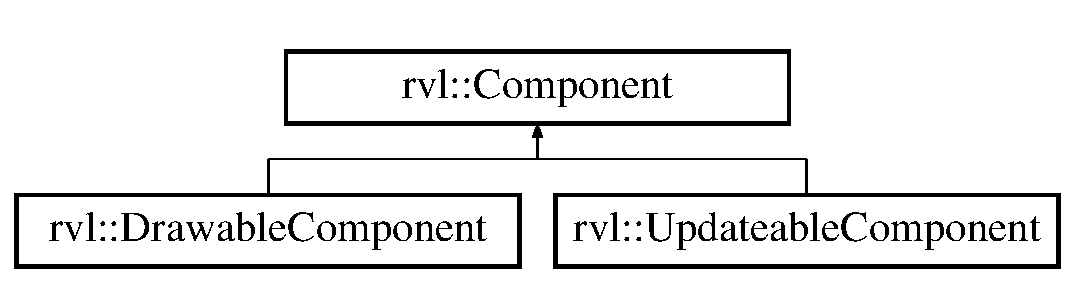
\includegraphics[height=2.000000cm]{classrvl_1_1_component}
\end{center}
\end{figure}
\subsection*{Public Member Functions}
\begin{DoxyCompactItemize}
\item 
\mbox{\Hypertarget{classrvl_1_1_component_a497f250d243d1c7de41c0bf4676903b1}\label{classrvl_1_1_component_a497f250d243d1c7de41c0bf4676903b1}} 
virtual void {\bfseries Awake} ()=0
\item 
\mbox{\Hypertarget{classrvl_1_1_component_ad3e6a3ef9492973b4df7770cc3cf92d2}\label{classrvl_1_1_component_ad3e6a3ef9492973b4df7770cc3cf92d2}} 
virtual void {\bfseries Start} ()=0
\item 
\mbox{\Hypertarget{classrvl_1_1_component_a85b9c9b9750440caf128b61afb20de4c}\label{classrvl_1_1_component_a85b9c9b9750440caf128b61afb20de4c}} 
virtual void {\bfseries On\+Destroy} ()=0
\end{DoxyCompactItemize}
\subsection*{Protected Attributes}
\begin{DoxyCompactItemize}
\item 
\mbox{\Hypertarget{classrvl_1_1_component_aa5cd621700ec5a36be00f9fbd9ef9b8f}\label{classrvl_1_1_component_aa5cd621700ec5a36be00f9fbd9ef9b8f}} 
bool {\bfseries destroy}
\end{DoxyCompactItemize}


\subsection{Detailed Description}
\hyperlink{classrvl_1_1_component}{Component} is an abstract base class for everything that can be attached to Game\+Objects. 

The documentation for this class was generated from the following file\+:\begin{DoxyCompactItemize}
\item 
Component/Component.\+h\end{DoxyCompactItemize}

\hypertarget{classrvl_1_1_drawable_component}{}\section{rvl\+:\+:Drawable\+Component Class Reference}
\label{classrvl_1_1_drawable_component}\index{rvl\+::\+Drawable\+Component@{rvl\+::\+Drawable\+Component}}
Inheritance diagram for rvl\+:\+:Drawable\+Component\+:\begin{figure}[H]
\begin{center}
\leavevmode
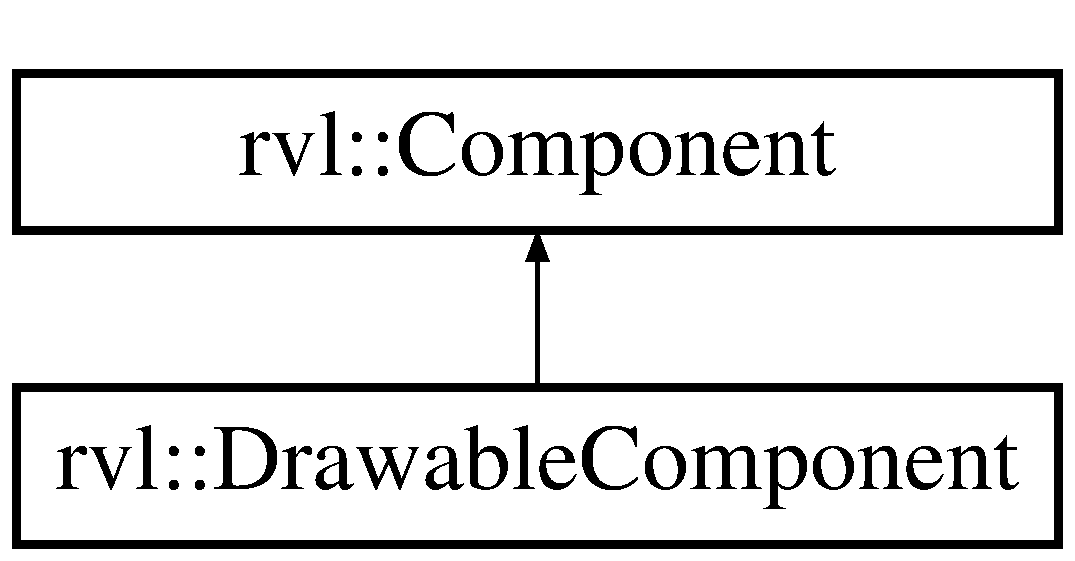
\includegraphics[height=2.000000cm]{classrvl_1_1_drawable_component}
\end{center}
\end{figure}
\subsection*{Public Member Functions}
\begin{DoxyCompactItemize}
\item 
\mbox{\Hypertarget{classrvl_1_1_drawable_component_a98aae95129af2f5c17ba9df97e7e954f}\label{classrvl_1_1_drawable_component_a98aae95129af2f5c17ba9df97e7e954f}} 
virtual void {\bfseries Draw} ()=0
\end{DoxyCompactItemize}
\subsection*{Additional Inherited Members}


The documentation for this class was generated from the following files\+:\begin{DoxyCompactItemize}
\item 
Component/Drawable\+Component.\+h\item 
Component/Drawable\+Component.\+cpp\end{DoxyCompactItemize}

\hypertarget{classrvl_1_1_game_object}{}\section{rvl\+:\+:Game\+Object Class Reference}
\label{classrvl_1_1_game_object}\index{rvl\+::\+Game\+Object@{rvl\+::\+Game\+Object}}
\subsection*{Public Member Functions}
\begin{DoxyCompactItemize}
\item 
\hyperlink{classrvl_1_1_game_object_a0348e3ee2e83d56eafca7a3547f432c4}{Game\+Object} ()
\item 
\mbox{\Hypertarget{classrvl_1_1_game_object_a6ad2b16e8f9e749ec2ee9598d4d3ae8d}\label{classrvl_1_1_game_object_a6ad2b16e8f9e749ec2ee9598d4d3ae8d}} 
{\bfseries Game\+Object} (\hyperlink{structrvl_1_1_shared_context}{rvl\+::\+Shared\+Context} $\ast$context)
\item 
\mbox{\Hypertarget{classrvl_1_1_game_object_a275a49882a7d619adef9698fee03fdab}\label{classrvl_1_1_game_object_a275a49882a7d619adef9698fee03fdab}} 
void {\bfseries Fixed\+Update} ()
\item 
\mbox{\Hypertarget{classrvl_1_1_game_object_a3d0364d2a33aaadb0a00e530bd7d54c3}\label{classrvl_1_1_game_object_a3d0364d2a33aaadb0a00e530bd7d54c3}} 
void {\bfseries Update} ()
\item 
\mbox{\Hypertarget{classrvl_1_1_game_object_a81751a7dfa6c0210449aa66fb731807c}\label{classrvl_1_1_game_object_a81751a7dfa6c0210449aa66fb731807c}} 
void {\bfseries Late\+Update} ()
\item 
\mbox{\Hypertarget{classrvl_1_1_game_object_a69e5c86216b242ae78efa64ffde2ac17}\label{classrvl_1_1_game_object_a69e5c86216b242ae78efa64ffde2ac17}} 
void {\bfseries Draw} ()
\item 
{\footnotesize template$<$typename T $>$ }\\T $\ast$ \hyperlink{classrvl_1_1_game_object_a84322da781cdc35cc352e4aaac5f9e47}{Get\+Component} () const
\begin{DoxyCompactList}\small\item\em T$\ast$ \hyperlink{classrvl_1_1_game_object_a84322da781cdc35cc352e4aaac5f9e47}{Get\+Component()} \end{DoxyCompactList}\item 
{\footnotesize template$<$typename T $>$ }\\T $\ast$ \hyperlink{classrvl_1_1_game_object_a84757644ca964d0f24e003d35bec60a7}{Add\+Component} ()
\begin{DoxyCompactList}\small\item\em T$\ast$ \hyperlink{classrvl_1_1_game_object_a84757644ca964d0f24e003d35bec60a7}{Add\+Component()} \end{DoxyCompactList}\item 
{\footnotesize template$<$typename T $>$ }\\void \hyperlink{classrvl_1_1_game_object_a4b91502ba7295337f55c832dea27cf67}{Add\+Component} (T $\ast$component)
\begin{DoxyCompactList}\small\item\em void \hyperlink{classrvl_1_1_game_object_a4b91502ba7295337f55c832dea27cf67}{Add\+Component(\+T$\ast$ component)} \end{DoxyCompactList}\item 
void \hyperlink{classrvl_1_1_game_object_adfe0989dce9c2bf40a2b940595d7f6e3}{Get\+Transform} ()
\begin{DoxyCompactList}\small\item\em Get the object transform. \end{DoxyCompactList}\item 
\mbox{\Hypertarget{classrvl_1_1_game_object_a07639eeda59c4469da56f52a4eefb8ad}\label{classrvl_1_1_game_object_a07639eeda59c4469da56f52a4eefb8ad}} 
\hyperlink{structrvl_1_1_shared_context}{rvl\+::\+Shared\+Context} $\ast$ {\bfseries Get\+Context} () const
\end{DoxyCompactItemize}


\subsection{Constructor \& Destructor Documentation}
\mbox{\Hypertarget{classrvl_1_1_game_object_a0348e3ee2e83d56eafca7a3547f432c4}\label{classrvl_1_1_game_object_a0348e3ee2e83d56eafca7a3547f432c4}} 
\index{rvl\+::\+Game\+Object@{rvl\+::\+Game\+Object}!Game\+Object@{Game\+Object}}
\index{Game\+Object@{Game\+Object}!rvl\+::\+Game\+Object@{rvl\+::\+Game\+Object}}
\subsubsection{\texorpdfstring{Game\+Object()}{GameObject()}}
{\footnotesize\ttfamily Game\+Object\+::\+Game\+Object (\begin{DoxyParamCaption}{ }\end{DoxyParamCaption})}

Base class for all types of objects in the Scenes. 

\subsection{Member Function Documentation}
\mbox{\Hypertarget{classrvl_1_1_game_object_a84757644ca964d0f24e003d35bec60a7}\label{classrvl_1_1_game_object_a84757644ca964d0f24e003d35bec60a7}} 
\index{rvl\+::\+Game\+Object@{rvl\+::\+Game\+Object}!Add\+Component@{Add\+Component}}
\index{Add\+Component@{Add\+Component}!rvl\+::\+Game\+Object@{rvl\+::\+Game\+Object}}
\subsubsection{\texorpdfstring{Add\+Component()}{AddComponent()}\hspace{0.1cm}{\footnotesize\ttfamily [1/2]}}
{\footnotesize\ttfamily template$<$typename T $>$ \\
T$\ast$ rvl\+::\+Game\+Object\+::\+Add\+Component (\begin{DoxyParamCaption}{ }\end{DoxyParamCaption})\hspace{0.3cm}{\ttfamily [inline]}}



T$\ast$ \hyperlink{classrvl_1_1_game_object_a84757644ca964d0f24e003d35bec60a7}{Add\+Component()} 

Add\+Component attempts to add a component to this gameobject, by first looking through the map to see if that type of component already exists. If the component type does not exist, it adds it to this gameobject and returns it. If the component type already exists it takes that component and returns it.

\begin{DoxyReturn}{Returns}
Added/found component. 
\end{DoxyReturn}
\mbox{\Hypertarget{classrvl_1_1_game_object_a4b91502ba7295337f55c832dea27cf67}\label{classrvl_1_1_game_object_a4b91502ba7295337f55c832dea27cf67}} 
\index{rvl\+::\+Game\+Object@{rvl\+::\+Game\+Object}!Add\+Component@{Add\+Component}}
\index{Add\+Component@{Add\+Component}!rvl\+::\+Game\+Object@{rvl\+::\+Game\+Object}}
\subsubsection{\texorpdfstring{Add\+Component()}{AddComponent()}\hspace{0.1cm}{\footnotesize\ttfamily [2/2]}}
{\footnotesize\ttfamily template$<$typename T $>$ \\
void rvl\+::\+Game\+Object\+::\+Add\+Component (\begin{DoxyParamCaption}\item[{T $\ast$}]{component }\end{DoxyParamCaption})\hspace{0.3cm}{\ttfamily [inline]}}



void \hyperlink{classrvl_1_1_game_object_a4b91502ba7295337f55c832dea27cf67}{Add\+Component(\+T$\ast$ component)} 

\hyperlink{classrvl_1_1_game_object_a4b91502ba7295337f55c832dea27cf67}{Add\+Component(\+T$\ast$ component)} attempts to add a component that was created outside this gameobject. \mbox{\Hypertarget{classrvl_1_1_game_object_a84322da781cdc35cc352e4aaac5f9e47}\label{classrvl_1_1_game_object_a84322da781cdc35cc352e4aaac5f9e47}} 
\index{rvl\+::\+Game\+Object@{rvl\+::\+Game\+Object}!Get\+Component@{Get\+Component}}
\index{Get\+Component@{Get\+Component}!rvl\+::\+Game\+Object@{rvl\+::\+Game\+Object}}
\subsubsection{\texorpdfstring{Get\+Component()}{GetComponent()}}
{\footnotesize\ttfamily template$<$typename T $>$ \\
T$\ast$ rvl\+::\+Game\+Object\+::\+Get\+Component (\begin{DoxyParamCaption}{ }\end{DoxyParamCaption}) const\hspace{0.3cm}{\ttfamily [inline]}}



T$\ast$ \hyperlink{classrvl_1_1_game_object_a84322da781cdc35cc352e4aaac5f9e47}{Get\+Component()} 

\hyperlink{classrvl_1_1_game_object_a84322da781cdc35cc352e4aaac5f9e47}{Get\+Component()} tries to find a component attached to this \hyperlink{classrvl_1_1_game_object}{Game\+Object}. If the \hyperlink{classrvl_1_1_component}{Component} is found it returns a pointer to it. Otherwise it returns nullptr.

\begin{DoxyReturn}{Returns}
Found component/nullptr. 
\end{DoxyReturn}
\mbox{\Hypertarget{classrvl_1_1_game_object_adfe0989dce9c2bf40a2b940595d7f6e3}\label{classrvl_1_1_game_object_adfe0989dce9c2bf40a2b940595d7f6e3}} 
\index{rvl\+::\+Game\+Object@{rvl\+::\+Game\+Object}!Get\+Transform@{Get\+Transform}}
\index{Get\+Transform@{Get\+Transform}!rvl\+::\+Game\+Object@{rvl\+::\+Game\+Object}}
\subsubsection{\texorpdfstring{Get\+Transform()}{GetTransform()}}
{\footnotesize\ttfamily void rvl\+::\+Game\+Object\+::\+Get\+Transform (\begin{DoxyParamCaption}{ }\end{DoxyParamCaption})}



Get the object transform. 

\begin{DoxyReturn}{Returns}
The transform of the gameobject. 
\end{DoxyReturn}


The documentation for this class was generated from the following files\+:\begin{DoxyCompactItemize}
\item 
Entity/Game\+Object.\+h\item 
Entity/Game\+Object.\+cpp\end{DoxyCompactItemize}

\hypertarget{classrvl_1_1_image_layer}{}\section{rvl\+:\+:Image\+Layer Class Reference}
\label{classrvl_1_1_image_layer}\index{rvl\+::\+Image\+Layer@{rvl\+::\+Image\+Layer}}


{\ttfamily \#include $<$Image\+Layer.\+h$>$}

Inheritance diagram for rvl\+:\+:Image\+Layer\+:\begin{figure}[H]
\begin{center}
\leavevmode
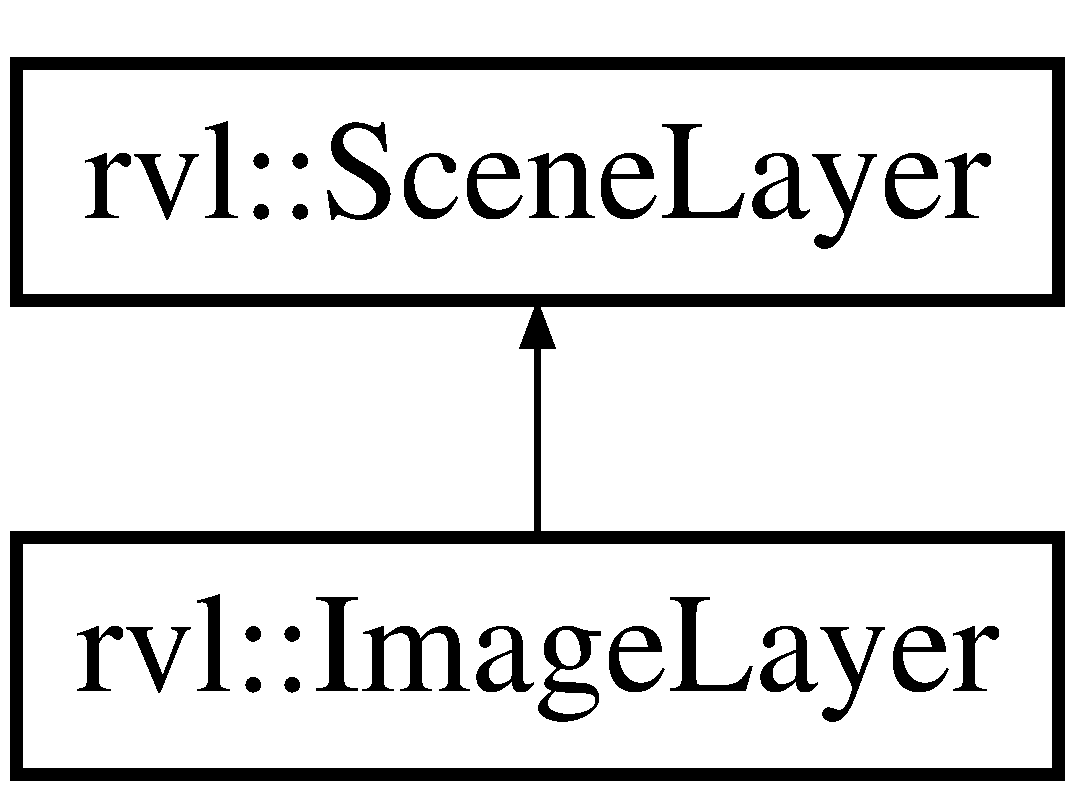
\includegraphics[height=2.000000cm]{classrvl_1_1_image_layer}
\end{center}
\end{figure}
\subsection*{Additional Inherited Members}


\subsection{Detailed Description}
\hyperlink{classrvl_1_1_image_layer}{Image\+Layer} handles and draws an imagelayer imported from tiled. 

The documentation for this class was generated from the following file\+:\begin{DoxyCompactItemize}
\item 
Graphics/Image\+Layer.\+h\end{DoxyCompactItemize}

\hypertarget{classrvl_1_1_object_layer}{}\section{rvl\+:\+:Object\+Layer Class Reference}
\label{classrvl_1_1_object_layer}\index{rvl\+::\+Object\+Layer@{rvl\+::\+Object\+Layer}}


{\ttfamily \#include $<$Object\+Layer.\+h$>$}

Inheritance diagram for rvl\+:\+:Object\+Layer\+:\begin{figure}[H]
\begin{center}
\leavevmode
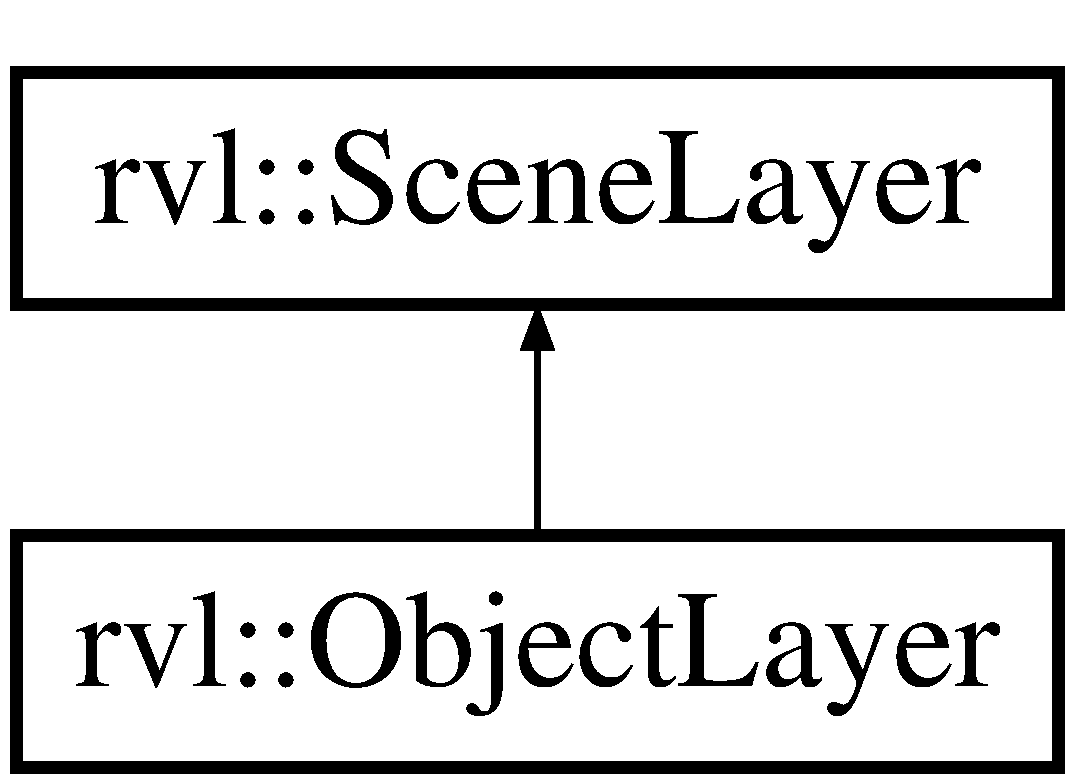
\includegraphics[height=2.000000cm]{classrvl_1_1_object_layer}
\end{center}
\end{figure}
\subsection*{Public Member Functions}
\begin{DoxyCompactItemize}
\item 
\mbox{\Hypertarget{classrvl_1_1_object_layer_a653283acf3afa9b685f3f888f8670a83}\label{classrvl_1_1_object_layer_a653283acf3afa9b685f3f888f8670a83}} 
{\bfseries Object\+Layer} (Tmx\+::\+Object\+Group $\ast$object\+Group, const std\+::vector$<$ sf\+::\+Texture $\ast$$>$ \&tilesets, \hyperlink{structrvl_1_1_shared_context}{rvl\+::\+Shared\+Context} $\ast$context)
\item 
virtual void \hyperlink{classrvl_1_1_object_layer_a3b29bd63ae4233eba84817bfe9eecae9}{Draw} (sf\+::\+Render\+Window \&window)
\begin{DoxyCompactList}\small\item\em Draw. \end{DoxyCompactList}\end{DoxyCompactItemize}


\subsection{Detailed Description}
\hyperlink{classrvl_1_1_object_layer}{Object\+Layer} translates all the objects from a Tmx\+::\+Object\+Group and adds them as gameobjects to the game. 

\subsection{Member Function Documentation}
\mbox{\Hypertarget{classrvl_1_1_object_layer_a3b29bd63ae4233eba84817bfe9eecae9}\label{classrvl_1_1_object_layer_a3b29bd63ae4233eba84817bfe9eecae9}} 
\index{rvl\+::\+Object\+Layer@{rvl\+::\+Object\+Layer}!Draw@{Draw}}
\index{Draw@{Draw}!rvl\+::\+Object\+Layer@{rvl\+::\+Object\+Layer}}
\subsubsection{\texorpdfstring{Draw()}{Draw()}}
{\footnotesize\ttfamily void rvl\+::\+Object\+Layer\+::\+Draw (\begin{DoxyParamCaption}\item[{sf\+::\+Render\+Window \&}]{window }\end{DoxyParamCaption})\hspace{0.3cm}{\ttfamily [virtual]}}



Draw. 

Sorts all gameobjects on this layer and then draws them out. 

Implements \hyperlink{classrvl_1_1_scene_layer}{rvl\+::\+Scene\+Layer}.



The documentation for this class was generated from the following files\+:\begin{DoxyCompactItemize}
\item 
Graphics/Object\+Layer.\+h\item 
Graphics/Object\+Layer.\+cpp\end{DoxyCompactItemize}

\hypertarget{classrvl_1_1_resource_manager}{}\section{rvl\+:\+:Resource\+Manager$<$ Derived, T $>$ Class Template Reference}
\label{classrvl_1_1_resource_manager}\index{rvl\+::\+Resource\+Manager$<$ Derived, T $>$@{rvl\+::\+Resource\+Manager$<$ Derived, T $>$}}


{\ttfamily \#include $<$Resource\+Manager.\+h$>$}

\subsection*{Protected Member Functions}
\begin{DoxyCompactItemize}
\item 
\mbox{\Hypertarget{classrvl_1_1_resource_manager_abdb9d99cc50e50a463432a4409b3cd46}\label{classrvl_1_1_resource_manager_abdb9d99cc50e50a463432a4409b3cd46}} 
T $\ast$ {\bfseries Load} (const std\+::string \&path)
\end{DoxyCompactItemize}


\subsection{Detailed Description}
\subsubsection*{template$<$typename Derived, typename T$>$\newline
class rvl\+::\+Resource\+Manager$<$ Derived, T $>$}

\hyperlink{classrvl_1_1_resource_manager}{Resource\+Manager} takes care of automated resource handling. It tracks the amount of objects/components that is requiring a specific resource, and removes the resource from memory when no object in the game needs it anymore. 

The documentation for this class was generated from the following file\+:\begin{DoxyCompactItemize}
\item 
Utils/Resource\+Manager.\+h\end{DoxyCompactItemize}

\hypertarget{classrvl_1_1_revel_game}{}\section{rvl\+:\+:Revel\+Game Class Reference}
\label{classrvl_1_1_revel_game}\index{rvl\+::\+Revel\+Game@{rvl\+::\+Revel\+Game}}


{\ttfamily \#include $<$Revel\+Game.\+h$>$}

\subsection*{Public Member Functions}
\begin{DoxyCompactItemize}
\item 
void \hyperlink{classrvl_1_1_revel_game_aaef0b7a8d82a7cc326b39f45c3be0b83}{Start} ()
\begin{DoxyCompactList}\small\item\em void \hyperlink{classrvl_1_1_revel_game_aaef0b7a8d82a7cc326b39f45c3be0b83}{Start()} \end{DoxyCompactList}\item 
void \hyperlink{classrvl_1_1_revel_game_ae2e535afe54176e266c1ec25ad11f9bc}{Stop} ()
\begin{DoxyCompactList}\small\item\em void \hyperlink{classrvl_1_1_revel_game_ae2e535afe54176e266c1ec25ad11f9bc}{Stop()} \end{DoxyCompactList}\item 
const \hyperlink{structrvl_1_1_shared_context}{Shared\+Context} \& \hyperlink{classrvl_1_1_revel_game_ab5f7b1a12844e3481d66ab00db1f0104}{Get\+Context} () const
\begin{DoxyCompactList}\small\item\em const \hyperlink{structrvl_1_1_shared_context}{Shared\+Context}\& \hyperlink{classrvl_1_1_revel_game_ab5f7b1a12844e3481d66ab00db1f0104}{Get\+Context() const} \end{DoxyCompactList}\end{DoxyCompactItemize}


\subsection{Detailed Description}
\hyperlink{classrvl_1_1_revel_game}{Revel\+Game} is the core of the engine. 

\subsection{Member Function Documentation}
\mbox{\Hypertarget{classrvl_1_1_revel_game_ab5f7b1a12844e3481d66ab00db1f0104}\label{classrvl_1_1_revel_game_ab5f7b1a12844e3481d66ab00db1f0104}} 
\index{rvl\+::\+Revel\+Game@{rvl\+::\+Revel\+Game}!Get\+Context@{Get\+Context}}
\index{Get\+Context@{Get\+Context}!rvl\+::\+Revel\+Game@{rvl\+::\+Revel\+Game}}
\subsubsection{\texorpdfstring{Get\+Context()}{GetContext()}}
{\footnotesize\ttfamily const \hyperlink{structrvl_1_1_shared_context}{Shared\+Context} \& rvl\+::\+Revel\+Game\+::\+Get\+Context (\begin{DoxyParamCaption}{ }\end{DoxyParamCaption}) const}



const \hyperlink{structrvl_1_1_shared_context}{Shared\+Context}\& \hyperlink{classrvl_1_1_revel_game_ab5f7b1a12844e3481d66ab00db1f0104}{Get\+Context() const} 

\begin{DoxyReturn}{Returns}
The games Context 
\end{DoxyReturn}
\mbox{\Hypertarget{classrvl_1_1_revel_game_aaef0b7a8d82a7cc326b39f45c3be0b83}\label{classrvl_1_1_revel_game_aaef0b7a8d82a7cc326b39f45c3be0b83}} 
\index{rvl\+::\+Revel\+Game@{rvl\+::\+Revel\+Game}!Start@{Start}}
\index{Start@{Start}!rvl\+::\+Revel\+Game@{rvl\+::\+Revel\+Game}}
\subsubsection{\texorpdfstring{Start()}{Start()}}
{\footnotesize\ttfamily void rvl\+::\+Revel\+Game\+::\+Start (\begin{DoxyParamCaption}{ }\end{DoxyParamCaption})}



void \hyperlink{classrvl_1_1_revel_game_aaef0b7a8d82a7cc326b39f45c3be0b83}{Start()} 

Starts the game \mbox{\Hypertarget{classrvl_1_1_revel_game_ae2e535afe54176e266c1ec25ad11f9bc}\label{classrvl_1_1_revel_game_ae2e535afe54176e266c1ec25ad11f9bc}} 
\index{rvl\+::\+Revel\+Game@{rvl\+::\+Revel\+Game}!Stop@{Stop}}
\index{Stop@{Stop}!rvl\+::\+Revel\+Game@{rvl\+::\+Revel\+Game}}
\subsubsection{\texorpdfstring{Stop()}{Stop()}}
{\footnotesize\ttfamily void rvl\+::\+Revel\+Game\+::\+Stop (\begin{DoxyParamCaption}{ }\end{DoxyParamCaption})}



void \hyperlink{classrvl_1_1_revel_game_ae2e535afe54176e266c1ec25ad11f9bc}{Stop()} 

Stops the game from running and closes the window. 

The documentation for this class was generated from the following files\+:\begin{DoxyCompactItemize}
\item 
App/Revel\+Game.\+h\item 
App/Revel\+Game.\+cpp\end{DoxyCompactItemize}

\hypertarget{classrvl_1_1_scene}{}\section{rvl\+:\+:Scene Class Reference}
\label{classrvl_1_1_scene}\index{rvl\+::\+Scene@{rvl\+::\+Scene}}
\subsection*{Public Member Functions}
\begin{DoxyCompactItemize}
\item 
\mbox{\Hypertarget{classrvl_1_1_scene_ae6675125abb9ee6dc2e1be81aef3e270}\label{classrvl_1_1_scene_ae6675125abb9ee6dc2e1be81aef3e270}} 
void {\bfseries Update} ()
\item 
\mbox{\Hypertarget{classrvl_1_1_scene_a62dd092ce10da061bb2bbb49eb0607db}\label{classrvl_1_1_scene_a62dd092ce10da061bb2bbb49eb0607db}} 
void {\bfseries Draw} (sf\+::\+Render\+Window \&window)
\item 
\mbox{\Hypertarget{classrvl_1_1_scene_ab871b7005408e83aaf2df91051338c5f}\label{classrvl_1_1_scene_ab871b7005408e83aaf2df91051338c5f}} 
bool {\bfseries Load} (std\+::string file\+Path)
\end{DoxyCompactItemize}


The documentation for this class was generated from the following files\+:\begin{DoxyCompactItemize}
\item 
Scene.\+h\item 
Scene.\+cpp\end{DoxyCompactItemize}

\hypertarget{classrvl_1_1_scene_layer}{}\section{rvl\+:\+:Scene\+Layer Class Reference}
\label{classrvl_1_1_scene_layer}\index{rvl\+::\+Scene\+Layer@{rvl\+::\+Scene\+Layer}}


\hyperlink{classrvl_1_1_scene_layer}{Scene\+Layer}.  




{\ttfamily \#include $<$Scene\+Layer.\+h$>$}

Inheritance diagram for rvl\+:\+:Scene\+Layer\+:\begin{figure}[H]
\begin{center}
\leavevmode
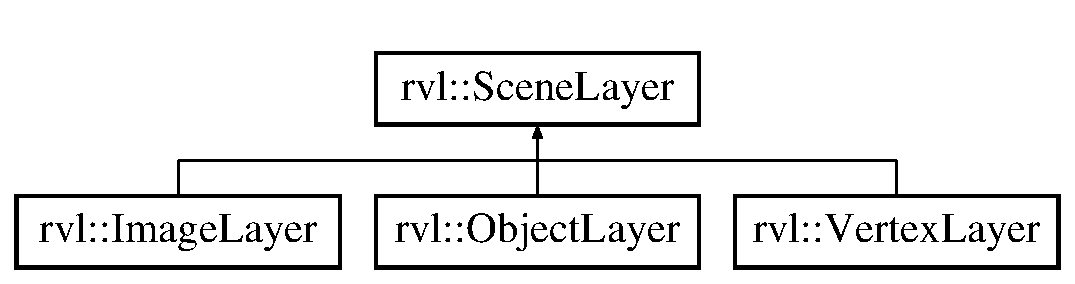
\includegraphics[height=2.000000cm]{classrvl_1_1_scene_layer}
\end{center}
\end{figure}
\subsection*{Public Member Functions}
\begin{DoxyCompactItemize}
\item 
\mbox{\Hypertarget{classrvl_1_1_scene_layer_aaaf36766d7c6990f82bad34c7c57259d}\label{classrvl_1_1_scene_layer_aaaf36766d7c6990f82bad34c7c57259d}} 
virtual void {\bfseries Draw} (sf\+::\+Render\+Window \&window)=0
\end{DoxyCompactItemize}


\subsection{Detailed Description}
\hyperlink{classrvl_1_1_scene_layer}{Scene\+Layer}. 

\hyperlink{classrvl_1_1_scene_layer}{Scene\+Layer} is an abstract class for all the types of layers available in tiled. 

The documentation for this class was generated from the following files\+:\begin{DoxyCompactItemize}
\item 
Graphics/Scene\+Layer.\+h\item 
Graphics/Scene\+Layer.\+cpp\end{DoxyCompactItemize}

\hypertarget{structrvl_1_1_shared_context}{}\section{rvl\+:\+:Shared\+Context Struct Reference}
\label{structrvl_1_1_shared_context}\index{rvl\+::\+Shared\+Context@{rvl\+::\+Shared\+Context}}


{\ttfamily \#include $<$Shared\+Context.\+h$>$}

\subsection*{Public Attributes}
\begin{DoxyCompactItemize}
\item 
\mbox{\Hypertarget{structrvl_1_1_shared_context_aa7cc22c51d90b03ebb095f204d138795}\label{structrvl_1_1_shared_context_aa7cc22c51d90b03ebb095f204d138795}} 
\hyperlink{classrvl_1_1_time}{Time} $\ast$ {\bfseries time}
\item 
\mbox{\Hypertarget{structrvl_1_1_shared_context_a616231b97cd2354f155598b77d76508d}\label{structrvl_1_1_shared_context_a616231b97cd2354f155598b77d76508d}} 
sf\+::\+Render\+Window $\ast$ {\bfseries window}
\item 
\mbox{\Hypertarget{structrvl_1_1_shared_context_a1011cf18940500204eecc4b4995a6bad}\label{structrvl_1_1_shared_context_a1011cf18940500204eecc4b4995a6bad}} 
lua\+\_\+\+State $\ast$ {\bfseries lua\+State}
\item 
\mbox{\Hypertarget{structrvl_1_1_shared_context_a6b2bbf356b1315eed46db97a49a9e559}\label{structrvl_1_1_shared_context_a6b2bbf356b1315eed46db97a49a9e559}} 
b2\+World $\ast$ {\bfseries physics\+World}
\end{DoxyCompactItemize}


\subsection{Detailed Description}
\hyperlink{structrvl_1_1_shared_context}{Shared\+Context} holds pointers to all types of context that is shared. 

The documentation for this struct was generated from the following file\+:\begin{DoxyCompactItemize}
\item 
Shared\+Context.\+h\end{DoxyCompactItemize}

\hypertarget{classrvl_1_1_time}{}\section{rvl\+:\+:Time Class Reference}
\label{classrvl_1_1_time}\index{rvl\+::\+Time@{rvl\+::\+Time}}
\subsection*{Public Member Functions}
\begin{DoxyCompactItemize}
\item 
\mbox{\Hypertarget{classrvl_1_1_time_ad22605375fc2a775f10fb80242fab9a7}\label{classrvl_1_1_time_ad22605375fc2a775f10fb80242fab9a7}} 
void {\bfseries Update} ()
\item 
const float \& \hyperlink{classrvl_1_1_time_a615b7d43aa2832dd6ffb235de22044cc}{Delta\+Time} () const
\begin{DoxyCompactList}\small\item\em const float\& \hyperlink{classrvl_1_1_time_a615b7d43aa2832dd6ffb235de22044cc}{Delta\+Time() const} \end{DoxyCompactList}\item 
const float \& \hyperlink{classrvl_1_1_time_a2edf11a18558efa227b3170eae433b3c}{Un\+Scaled\+Delta\+Time} () const
\begin{DoxyCompactList}\small\item\em const float\& \hyperlink{classrvl_1_1_time_a2edf11a18558efa227b3170eae433b3c}{Un\+Scaled\+Delta\+Time() const} \end{DoxyCompactList}\item 
void \hyperlink{classrvl_1_1_time_a6033a29cb79140a95337f78fe3de4f8a}{Set\+Time\+Scale} (const float \&time\+Scale)
\begin{DoxyCompactList}\small\item\em void \hyperlink{classrvl_1_1_time_a6033a29cb79140a95337f78fe3de4f8a}{Set\+Time\+Scale(const float\&)} \end{DoxyCompactList}\item 
const float \& \hyperlink{classrvl_1_1_time_adc601517b317a98bc72a1dd87826ae4e}{Get\+Time\+Scale} () const
\begin{DoxyCompactList}\small\item\em const float\& \hyperlink{classrvl_1_1_time_adc601517b317a98bc72a1dd87826ae4e}{Get\+Time\+Scale() const} \end{DoxyCompactList}\end{DoxyCompactItemize}


\subsection{Member Function Documentation}
\mbox{\Hypertarget{classrvl_1_1_time_a615b7d43aa2832dd6ffb235de22044cc}\label{classrvl_1_1_time_a615b7d43aa2832dd6ffb235de22044cc}} 
\index{rvl\+::\+Time@{rvl\+::\+Time}!Delta\+Time@{Delta\+Time}}
\index{Delta\+Time@{Delta\+Time}!rvl\+::\+Time@{rvl\+::\+Time}}
\subsubsection{\texorpdfstring{Delta\+Time()}{DeltaTime()}}
{\footnotesize\ttfamily const float \& rvl\+::\+Time\+::\+Delta\+Time (\begin{DoxyParamCaption}{ }\end{DoxyParamCaption}) const}



const float\& \hyperlink{classrvl_1_1_time_a615b7d43aa2832dd6ffb235de22044cc}{Delta\+Time() const} 

\begin{DoxyReturn}{Returns}
The deltatime based on timescale. 
\end{DoxyReturn}
\mbox{\Hypertarget{classrvl_1_1_time_adc601517b317a98bc72a1dd87826ae4e}\label{classrvl_1_1_time_adc601517b317a98bc72a1dd87826ae4e}} 
\index{rvl\+::\+Time@{rvl\+::\+Time}!Get\+Time\+Scale@{Get\+Time\+Scale}}
\index{Get\+Time\+Scale@{Get\+Time\+Scale}!rvl\+::\+Time@{rvl\+::\+Time}}
\subsubsection{\texorpdfstring{Get\+Time\+Scale()}{GetTimeScale()}}
{\footnotesize\ttfamily const float \& rvl\+::\+Time\+::\+Get\+Time\+Scale (\begin{DoxyParamCaption}{ }\end{DoxyParamCaption}) const}



const float\& \hyperlink{classrvl_1_1_time_adc601517b317a98bc72a1dd87826ae4e}{Get\+Time\+Scale() const} 

\begin{DoxyReturn}{Returns}
The timescale. 
\end{DoxyReturn}
\mbox{\Hypertarget{classrvl_1_1_time_a6033a29cb79140a95337f78fe3de4f8a}\label{classrvl_1_1_time_a6033a29cb79140a95337f78fe3de4f8a}} 
\index{rvl\+::\+Time@{rvl\+::\+Time}!Set\+Time\+Scale@{Set\+Time\+Scale}}
\index{Set\+Time\+Scale@{Set\+Time\+Scale}!rvl\+::\+Time@{rvl\+::\+Time}}
\subsubsection{\texorpdfstring{Set\+Time\+Scale()}{SetTimeScale()}}
{\footnotesize\ttfamily void rvl\+::\+Time\+::\+Set\+Time\+Scale (\begin{DoxyParamCaption}\item[{const float \&}]{time\+Scale }\end{DoxyParamCaption})}



void \hyperlink{classrvl_1_1_time_a6033a29cb79140a95337f78fe3de4f8a}{Set\+Time\+Scale(const float\&)} 

Set the timescale to the specified value. \mbox{\Hypertarget{classrvl_1_1_time_a2edf11a18558efa227b3170eae433b3c}\label{classrvl_1_1_time_a2edf11a18558efa227b3170eae433b3c}} 
\index{rvl\+::\+Time@{rvl\+::\+Time}!Un\+Scaled\+Delta\+Time@{Un\+Scaled\+Delta\+Time}}
\index{Un\+Scaled\+Delta\+Time@{Un\+Scaled\+Delta\+Time}!rvl\+::\+Time@{rvl\+::\+Time}}
\subsubsection{\texorpdfstring{Un\+Scaled\+Delta\+Time()}{UnScaledDeltaTime()}}
{\footnotesize\ttfamily const float \& rvl\+::\+Time\+::\+Un\+Scaled\+Delta\+Time (\begin{DoxyParamCaption}{ }\end{DoxyParamCaption}) const}



const float\& \hyperlink{classrvl_1_1_time_a2edf11a18558efa227b3170eae433b3c}{Un\+Scaled\+Delta\+Time() const} 

\begin{DoxyReturn}{Returns}
Deltatime without applying timescale. 
\end{DoxyReturn}


The documentation for this class was generated from the following files\+:\begin{DoxyCompactItemize}
\item 
Utils/Time.\+h\item 
Utils/Time.\+cpp\end{DoxyCompactItemize}

\hypertarget{classrvl_1_1_updateable_component}{}\section{rvl\+:\+:Updateable\+Component Class Reference}
\label{classrvl_1_1_updateable_component}\index{rvl\+::\+Updateable\+Component@{rvl\+::\+Updateable\+Component}}
Inheritance diagram for rvl\+:\+:Updateable\+Component\+:\begin{figure}[H]
\begin{center}
\leavevmode
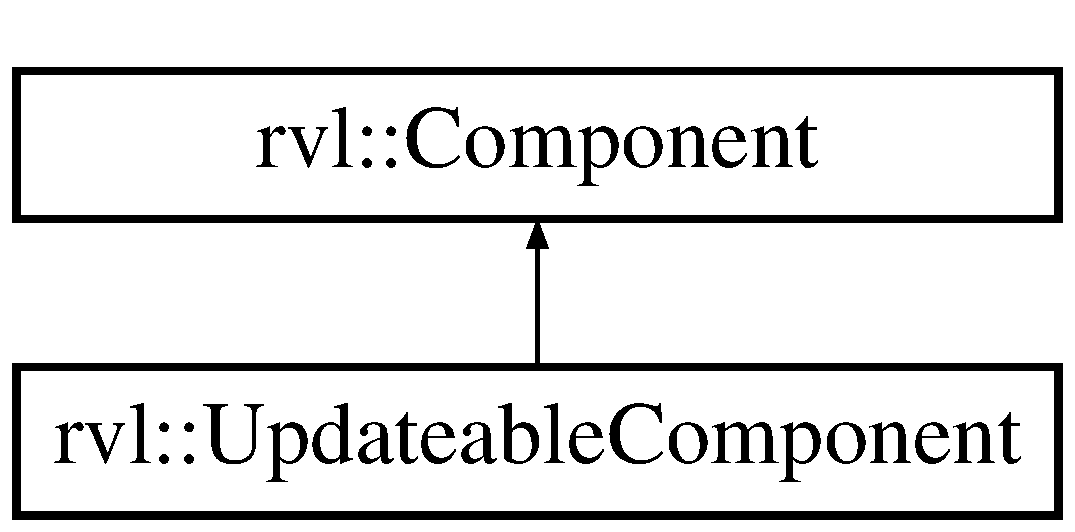
\includegraphics[height=2.000000cm]{classrvl_1_1_updateable_component}
\end{center}
\end{figure}
\subsection*{Public Member Functions}
\begin{DoxyCompactItemize}
\item 
\mbox{\Hypertarget{classrvl_1_1_updateable_component_a2fe539ca7ce0f7e54377e0c4fd0757fc}\label{classrvl_1_1_updateable_component_a2fe539ca7ce0f7e54377e0c4fd0757fc}} 
virtual void {\bfseries Fixed\+Update} ()=0
\item 
\mbox{\Hypertarget{classrvl_1_1_updateable_component_ac57d1edb8c648fd12447bbb1dd8411d3}\label{classrvl_1_1_updateable_component_ac57d1edb8c648fd12447bbb1dd8411d3}} 
virtual void {\bfseries Update} ()=0
\end{DoxyCompactItemize}
\subsection*{Additional Inherited Members}


The documentation for this class was generated from the following files\+:\begin{DoxyCompactItemize}
\item 
Component/Updateable\+Component.\+h\item 
Component/Updateable\+Component.\+cpp\end{DoxyCompactItemize}

\hypertarget{classrvl_1_1_vertex_layer}{}\section{rvl\+:\+:Vertex\+Layer Class Reference}
\label{classrvl_1_1_vertex_layer}\index{rvl\+::\+Vertex\+Layer@{rvl\+::\+Vertex\+Layer}}


{\ttfamily \#include $<$Vertex\+Layer.\+h$>$}

Inheritance diagram for rvl\+:\+:Vertex\+Layer\+:\begin{figure}[H]
\begin{center}
\leavevmode
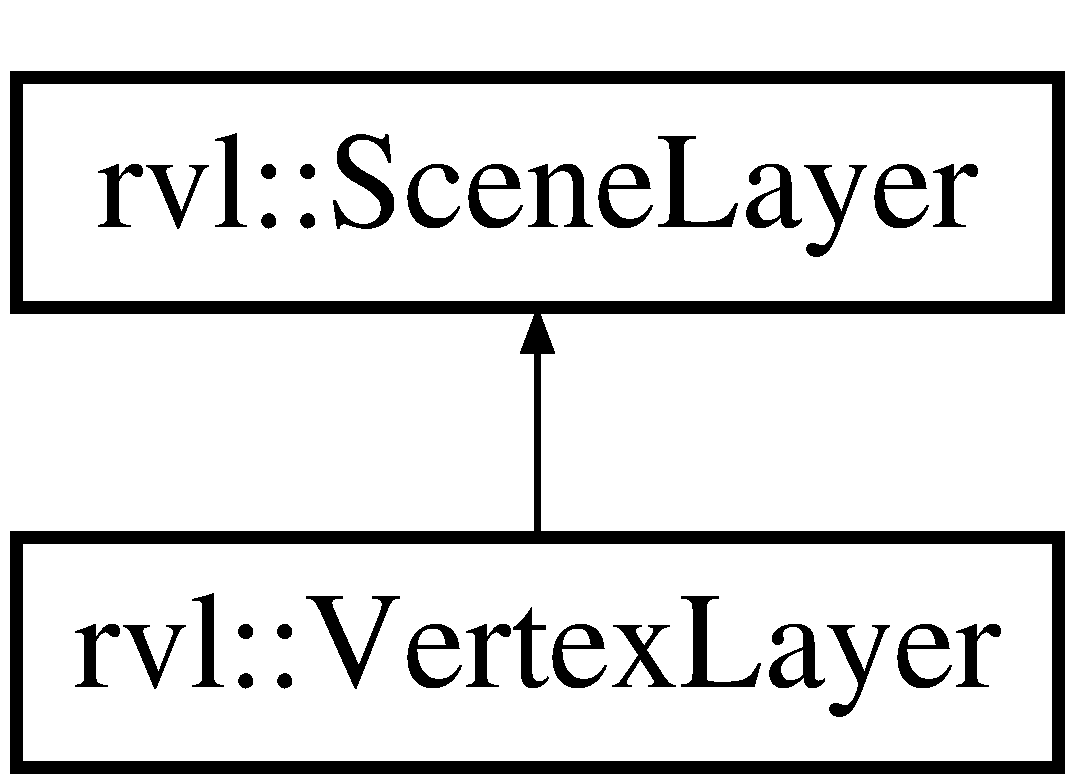
\includegraphics[height=2.000000cm]{classrvl_1_1_vertex_layer}
\end{center}
\end{figure}
\subsection*{Public Member Functions}
\begin{DoxyCompactItemize}
\item 
\mbox{\Hypertarget{classrvl_1_1_vertex_layer_aa6b21bdf5910c1afba2b6080f7555d64}\label{classrvl_1_1_vertex_layer_aa6b21bdf5910c1afba2b6080f7555d64}} 
{\bfseries Vertex\+Layer} (Tmx\+::\+Tile\+Layer $\ast$layer, int tile\+Width, int tile\+Height, std\+::vector$<$ sf\+::\+Texture $\ast$$>$ \&tileset)
\item 
void \hyperlink{classrvl_1_1_vertex_layer_aa6c20822af0bcbf0c57329348b92c0b4}{Draw} (sf\+::\+Render\+Window \&window) override
\begin{DoxyCompactList}\small\item\em Draw. \end{DoxyCompactList}\end{DoxyCompactItemize}


\subsection{Detailed Description}
\hyperlink{classrvl_1_1_vertex_layer}{Vertex\+Layer} is responsible for drawing out a Tmx\+::\+Tile\+Layer 

\subsection{Member Function Documentation}
\mbox{\Hypertarget{classrvl_1_1_vertex_layer_aa6c20822af0bcbf0c57329348b92c0b4}\label{classrvl_1_1_vertex_layer_aa6c20822af0bcbf0c57329348b92c0b4}} 
\index{rvl\+::\+Vertex\+Layer@{rvl\+::\+Vertex\+Layer}!Draw@{Draw}}
\index{Draw@{Draw}!rvl\+::\+Vertex\+Layer@{rvl\+::\+Vertex\+Layer}}
\subsubsection{\texorpdfstring{Draw()}{Draw()}}
{\footnotesize\ttfamily void rvl\+::\+Vertex\+Layer\+::\+Draw (\begin{DoxyParamCaption}\item[{sf\+::\+Render\+Window \&}]{window }\end{DoxyParamCaption})\hspace{0.3cm}{\ttfamily [override]}, {\ttfamily [virtual]}}



Draw. 

Draws all the Vertex\+Arrays to a specified sf\+::\+Render\+Window 

Implements \hyperlink{classrvl_1_1_scene_layer}{rvl\+::\+Scene\+Layer}.



The documentation for this class was generated from the following files\+:\begin{DoxyCompactItemize}
\item 
Graphics/Vertex\+Layer.\+h\item 
Graphics/Vertex\+Layer.\+cpp\end{DoxyCompactItemize}

\hypertarget{classrvl_1_1_window}{}\section{rvl\+:\+:Window Class Reference}
\label{classrvl_1_1_window}\index{rvl\+::\+Window@{rvl\+::\+Window}}
\subsection*{Public Member Functions}
\begin{DoxyCompactItemize}
\item 
\mbox{\Hypertarget{classrvl_1_1_window_afdd7957b70cc47072c521e5a3f4affb8}\label{classrvl_1_1_window_afdd7957b70cc47072c521e5a3f4affb8}} 
bool {\bfseries Create} (sf\+::\+Vector2u size, const char $\ast$title, bool full\+Screen)
\item 
\mbox{\Hypertarget{classrvl_1_1_window_adf0dfa18d5d6f180ea0e05b34903a657}\label{classrvl_1_1_window_adf0dfa18d5d6f180ea0e05b34903a657}} 
const sf\+::\+Vector2u \& {\bfseries Get\+Size} () const
\item 
\mbox{\Hypertarget{classrvl_1_1_window_a7a929cc1744c3b2548be9bbc4166e205}\label{classrvl_1_1_window_a7a929cc1744c3b2548be9bbc4166e205}} 
const uint32 \& {\bfseries Get\+Width} () const
\item 
\mbox{\Hypertarget{classrvl_1_1_window_acca4f280ab176716aef954e14ee5c2d4}\label{classrvl_1_1_window_acca4f280ab176716aef954e14ee5c2d4}} 
const uint32 \& {\bfseries Get\+Height} () const
\end{DoxyCompactItemize}


The documentation for this class was generated from the following file\+:\begin{DoxyCompactItemize}
\item 
Graphics/Window.\+h\end{DoxyCompactItemize}

%--- End generated contents ---

% Index
\backmatter
\newpage
\phantomsection
\clearemptydoublepage
\addcontentsline{toc}{chapter}{Index}
\printindex

\end{document}
